\chapter{Proposed calibration method}
\label{sec:proposed_calibration_method}




% ---------------------------------------------------------------
\section{Intrinsic Calibration}
\label{sec:intrinsic_calibration}
% ---------------------------------------------------------------

Intrinsic calibration is the first and foundational step of the overall
calibration pipeline. It estimates the internal optical parameters of the
camera — the intrinsic matrix $\mathbf{K}$ and the lens distortion
coefficients — which describe the mapping between three-dimensional points in
the camera coordinate frame and their projection onto the image plane
(Section~\ref{subsec:intrinsics}). Accurate intrinsic calibration is essential
for reliable pose estimation: any error in $\mathbf{K}$ directly propagates
into the PnP solution and, consequently, corrupts the
camera motion matrices $\mathbf{B}_{ij}$ used in hand-eye calibration
\cite{zhang2000flexible, hartley2004multiple}.

% ---------------------------------------------------------------
\subsection{Calibration Target Definition}
\label{subsec:intr_target}
% ---------------------------------------------------------------

The same rigid metallic ChArUco board described in
Section~\ref{subsec:calibration_target} is used for intrinsic calibration.
Its physical dimensions ($262 \times 402.5$\,mm), square size
($\approx 17.5$\,mm), and marker size ($\approx 12$\,mm) define a set of
reference 3D points $\{\mathbf{P}_j\}$ with known coordinates in the target
frame $\{T\}$, all lying on the plane $Z_T = 0$.

\begin{figure}[htbp]
	\centering
	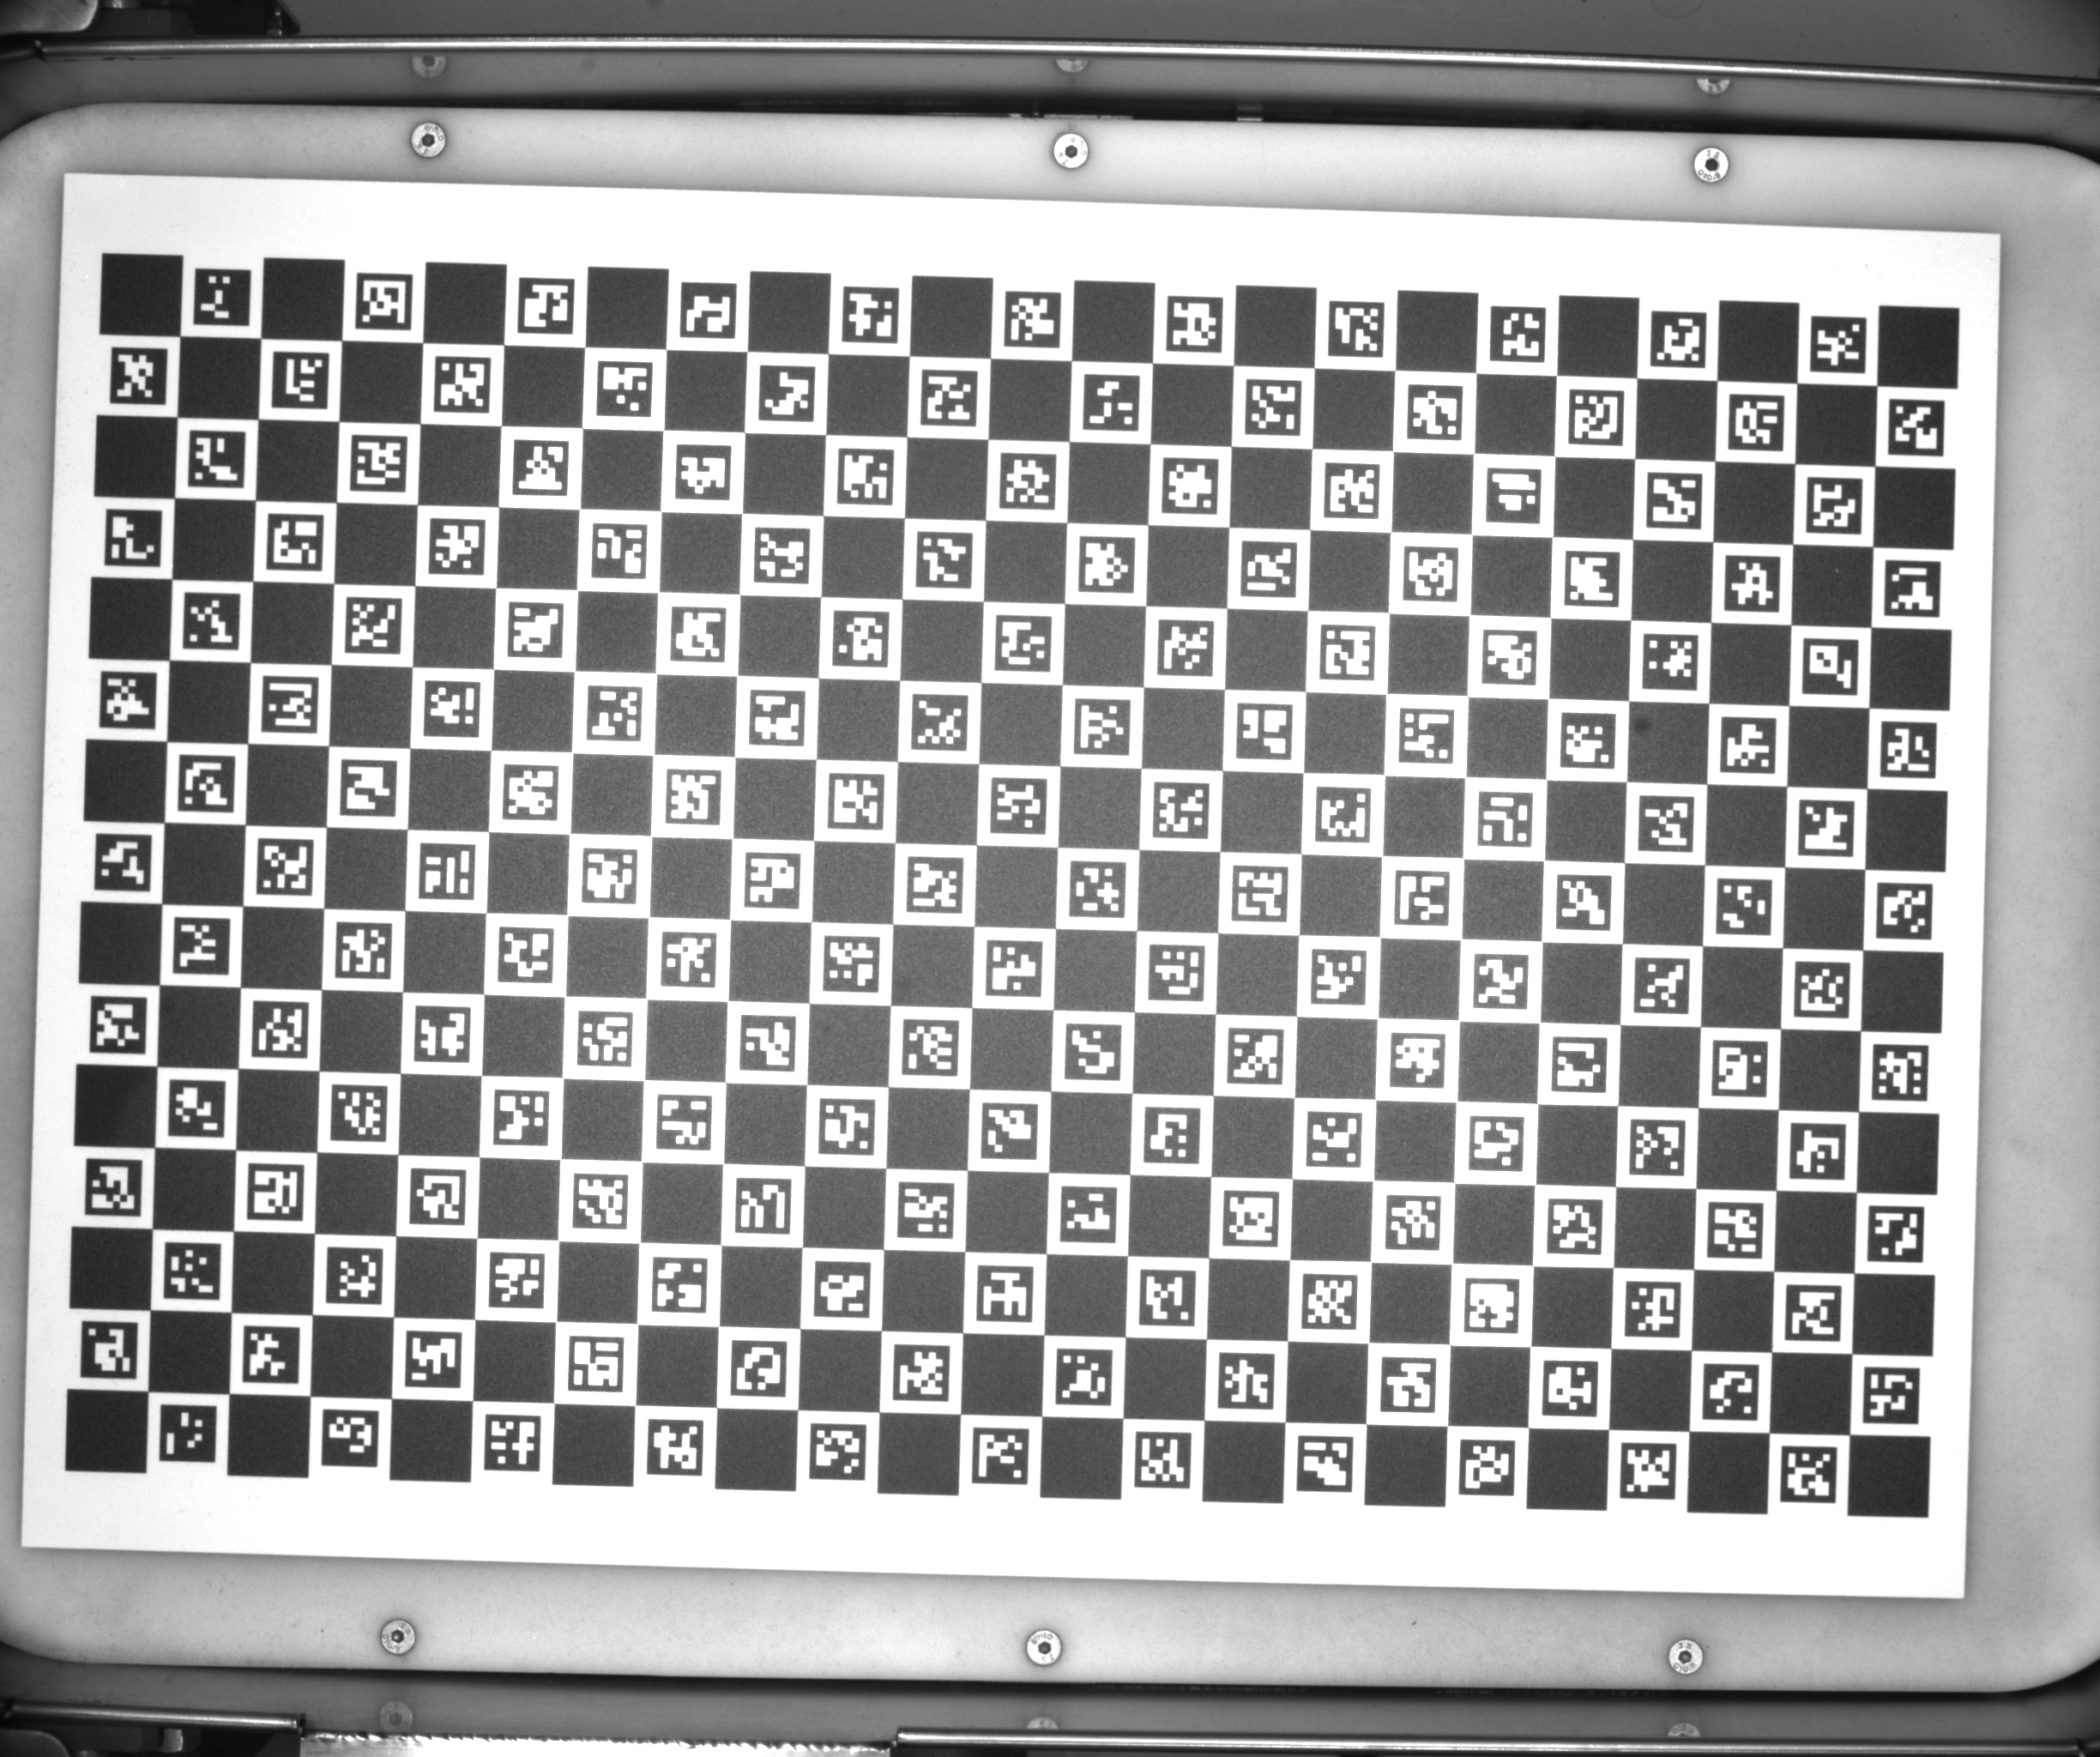
\includegraphics[width=0.42\linewidth]
	{images/chapter4Images/chessboardVertical.png}
	\caption{Rigid metallic ChArUco board used for intrinsic and hand-eye
		calibration. The board combines a checkerboard pattern with embedded
		ArUco markers, enabling robust corner identification and sub-pixel
		localization under partial occlusions and perspective distortion.}
	\label{fig:charuco_board_intrinsic}
\end{figure}

Using the same board for both intrinsic and hand-eye calibration has a
practical advantage: the same detection and pose estimation code path is
shared, eliminating any systematic bias that would arise from switching between
different targets. Furthermore, the rigidity of the metallic substrate
guarantees dimensional stability across temperature changes, avoiding the
planar deformation that can affect printed paper targets and introduce
systematic errors in the estimated intrinsic parameters \cite{garrido2014aruco}.

% ---------------------------------------------------------------
\subsection{Corner Detection and Refinement}
\label{subsec:intr_detection}
% ---------------------------------------------------------------

Feature extraction from each calibration image follows the three-stage
ChArUco detection pipeline described in Section~\ref{subsec:feature_detection}.
For intrinsic calibration, the same procedure is applied but without an initial
estimate of $\mathbf{K}$, so the ChArUco corner interpolation falls back to
the homography-based mode provided by OpenCV \cite{bradski2008learning}.

After the three detection stages, each accepted image $i$ contributes a set
of $m_i$ correspondences:

\begin{equation}
    \left\{
        \left(\tilde{\mathbf{p}}_j^{(i)},\; \mathbf{P}_j\right)
    \right\}_{j=1}^{m_i}
    \label{eq:correspondences}
\end{equation}

\noindent where $\tilde{\mathbf{p}}_j^{(i)} \in \mathbb{R}^2$ are the
refined sub-pixel image coordinates and $\mathbf{P}_j \in \mathbb{R}^3$ are
the known 3D board coordinates.

\begin{figure}[htbp]
	\centering
	
	\begin{subfigure}{0.62\linewidth}
		\centering
		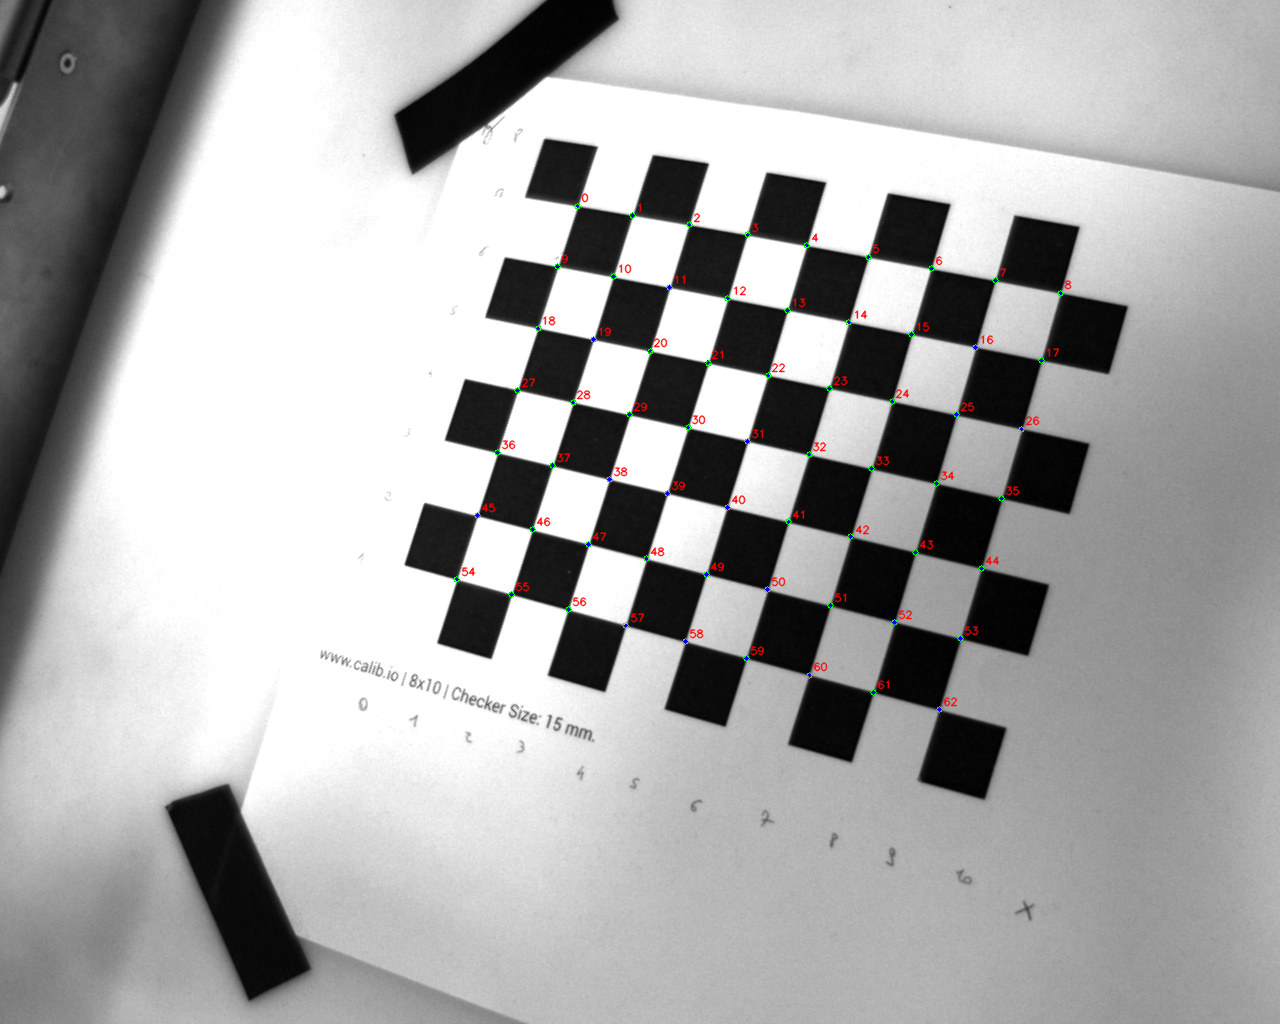
\includegraphics[width=\linewidth]
		{images/chapter4Images/pose_021.png}
		\caption{Full calibration image showing detected and reprojected
			feature points used during intrinsic calibration.}
		\label{fig:intrinsic_reprojection_full}
	\end{subfigure}
	\hfill
	\begin{subfigure}{0.34\linewidth}
		\centering
		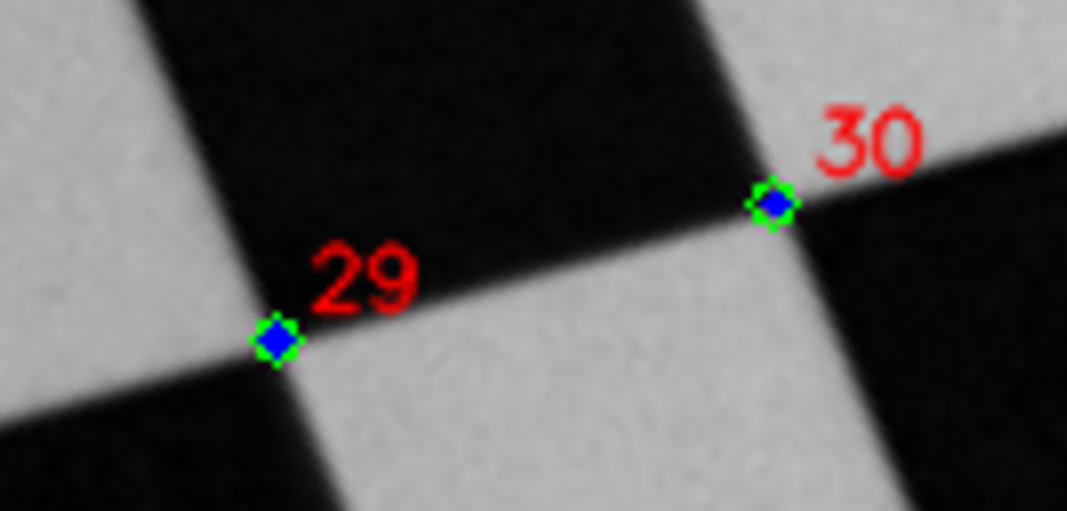
\includegraphics[width=\linewidth]
		{images/chapter4Images/pose_021_particular.png}
		\caption{Zoomed-in detail showing the detected corner (blue)
			and the corresponding reprojected corner (green).}
		\label{fig:intrinsic_reprojection_zoom}
	\end{subfigure}
	
	\caption{Example of corner detection and reprojection during intrinsic
		calibration. The close alignment between observed and reprojected points
		indicates low reprojection error and accurate estimation of the intrinsic
		camera parameters.}
	\label{fig:intrinsic_reprojection}
\end{figure}


Images are accepted only if $m_i \geq m_{\min}$, where $m_{\min}$ is set
to ensure that the resulting linear system is sufficiently over-determined.
In practice, a minimum of 5 corners per image is required by OpenCV's
\texttt{calibrateCamera()}, but a value of $m_{\min} = 8$ is preferably used in this
work to improve numerical conditioning.

% ---------------------------------------------------------------
\subsection{Calibration Procedure}
\label{subsec:intr_procedure}
% ---------------------------------------------------------------

Given $n$ accepted images with correspondence sets~\eqref{eq:correspondences},
intrinsic calibration simultaneously estimates:

\begin{itemize}
    \item the camera intrinsic matrix $\mathbf{K}$ (equation~\eqref{eq:camera_matrix}),
    parameterised by $(f_x, f_y, c_x, c_y)$ with skew $s = 0$ assumed;
    \item the distortion coefficient vector
    $\mathbf{d} = (k_1, k_2, p_1, p_2, k_3)^{\top}$
    (equations~\eqref{eq:radial_distortion}--\eqref{eq:tangential_distortion});
    \item a set of $n$ extrinsic poses
    $\{{}^C_T\mathbf{T}^{(i)}\}_{i=1}^n$, one per image, treated as nuisance
    parameters during instrinsic calibration.
\end{itemize}
\noindent The estimation is performed by minimising the total reprojection
error over all images and all detected corners:

TODO check argmin
\begin{equation}
    \left(\mathbf{K}^*, \mathbf{d}^*, \{{}^C_T\mathbf{T}^{(i)*}\}\right) =
    \operatorname*{arg\min}_{\mathbf{K},\, \mathbf{d},\, \{{}^C_T\mathbf{T}^{(i)}\}}
    \sum_{i=1}^{n} \sum_{j=1}^{m_i}
    \left\lVert
        \tilde{\mathbf{p}}_j^{(i)} -
        \pi\!\left(\mathbf{K},\, \mathbf{d},\,
        {}^C_T\mathbf{T}^{(i)},\, \mathbf{P}_j\right)
    \right\rVert^2
    \label{eq:calib_optim}
\end{equation}

\noindent where $\pi(\cdot)$ is the full projection function including lens
distortion (equation~\eqref{eq:projection}). The optimisation is initialised
using the closed-form homography-based method of Zhang \cite{zhang2000flexible}, as implemented
in \texttt{cv::calibrateCamera()} \cite{bradski2008learning}.

For ChArUco boards, the calibration can equivalently be performed using
\texttt{cv::aruco::calibrateCameraCharuco()}, which internally calls
\texttt{calibrateCamera()} on the interpolated corner set. Both functions
return the same intrinsic parameters $(\mathbf{K}^*, \mathbf{d}^*)$ and produce equivalent results;
the ChArUco-specific variant is preferred in this work because it performs
the corner interpolation and calibration in a single call.

Images are collected from a range of viewpoints, with the camera tilted relative to the board and
rotated to cover a wide variety of poses. This diversity is necessary because:

\begin{itemize}
    \item \textbf{Focal length and principal point} are best constrained by
    varying the distance between camera and board.
    \item \textbf{Radial distortion coefficients} are best constrained by
    including views where board corners appear near the edges of the image.
    \item \textbf{Tangential distortion coefficients} are best constrained
    by in-plane rotations of the camera relative to the board.
\end{itemize}

\noindent In this work, $n = 15$--$20$ images are used for calibration,
consistent with established guidelines \cite{zhang2000flexible,
hartley2004multiple}.

% ---------------------------------------------------------------
\subsection{Reprojection Error and Quality Assessment}
\label{subsec:intr_reproj}
% ---------------------------------------------------------------

The quality of the intrinsic calibration is evaluated using the
\textit{root mean square reprojection error} (RMS-RPE), defined as:

\begin{equation}
    \text{RMS-RPE} =
    \sqrt{
        \frac{1}{\sum_{i=1}^{n} m_i}
        \sum_{i=1}^{n} \sum_{j=1}^{m_i}
        \left\lVert
            \tilde{\mathbf{p}}_j^{(i)} -
            \pi\!\left(\mathbf{K}^*,\, \mathbf{d}^*,\,
            {}^C_T\mathbf{T}^{(i)*},\, \mathbf{P}_j\right)
        \right\rVert^2
    }
    \label{eq:rms_rpe}
\end{equation}

\noindent expressed in pixel units. The RMS-RPE measures the average distance
between the detected corner positions and the positions predicted by the
calibrated camera model. A well-calibrated camera with a 12\,MP sensor at a
working distance of 30--40\,cm typically achieves a
$\text{RMS-RPE}$\, in the range of 0.4–1.0 px for high-quality industrial setups, depending on sensor resolution and setup stability \cite{zhang2000flexible}.

In addition to the global RMS-RPE, a per-image reprojection error is computed:

\begin{equation}
    \bar{\epsilon}^{(i)} =
    \frac{1}{m_i}
    \sum_{j=1}^{m_i}
    \left\lVert
        \tilde{\mathbf{p}}_j^{(i)} -
        \pi\!\left(\mathbf{K}^*,\, \mathbf{d}^*,\,
        {}^C_T\mathbf{T}^{(i)*},\, \mathbf{P}_j\right)
    \right\rVert
    \label{eq:per_image_rpe}
\end{equation}

\noindent Images with $\bar{\epsilon}^{(i)}$ significantly above the mean
are treated as outliers and removed from the dataset. The calibration is then
re-run on the filtered set until the per-image errors are uniformly
distributed, with no single image dominating the total error budget. This
iterative outlier rejection strategy improves the stability of the final
intrinsic estimate.

The estimated intrinsic parameters $(\mathbf{K}^*, \mathbf{d}^*)$ obtained
from this procedure are stored and used in all subsequent stages: ChArUco
corner interpolation, pose estimation, and hand-eye calibration.

\begin{figure}[htbp]
	\centering
	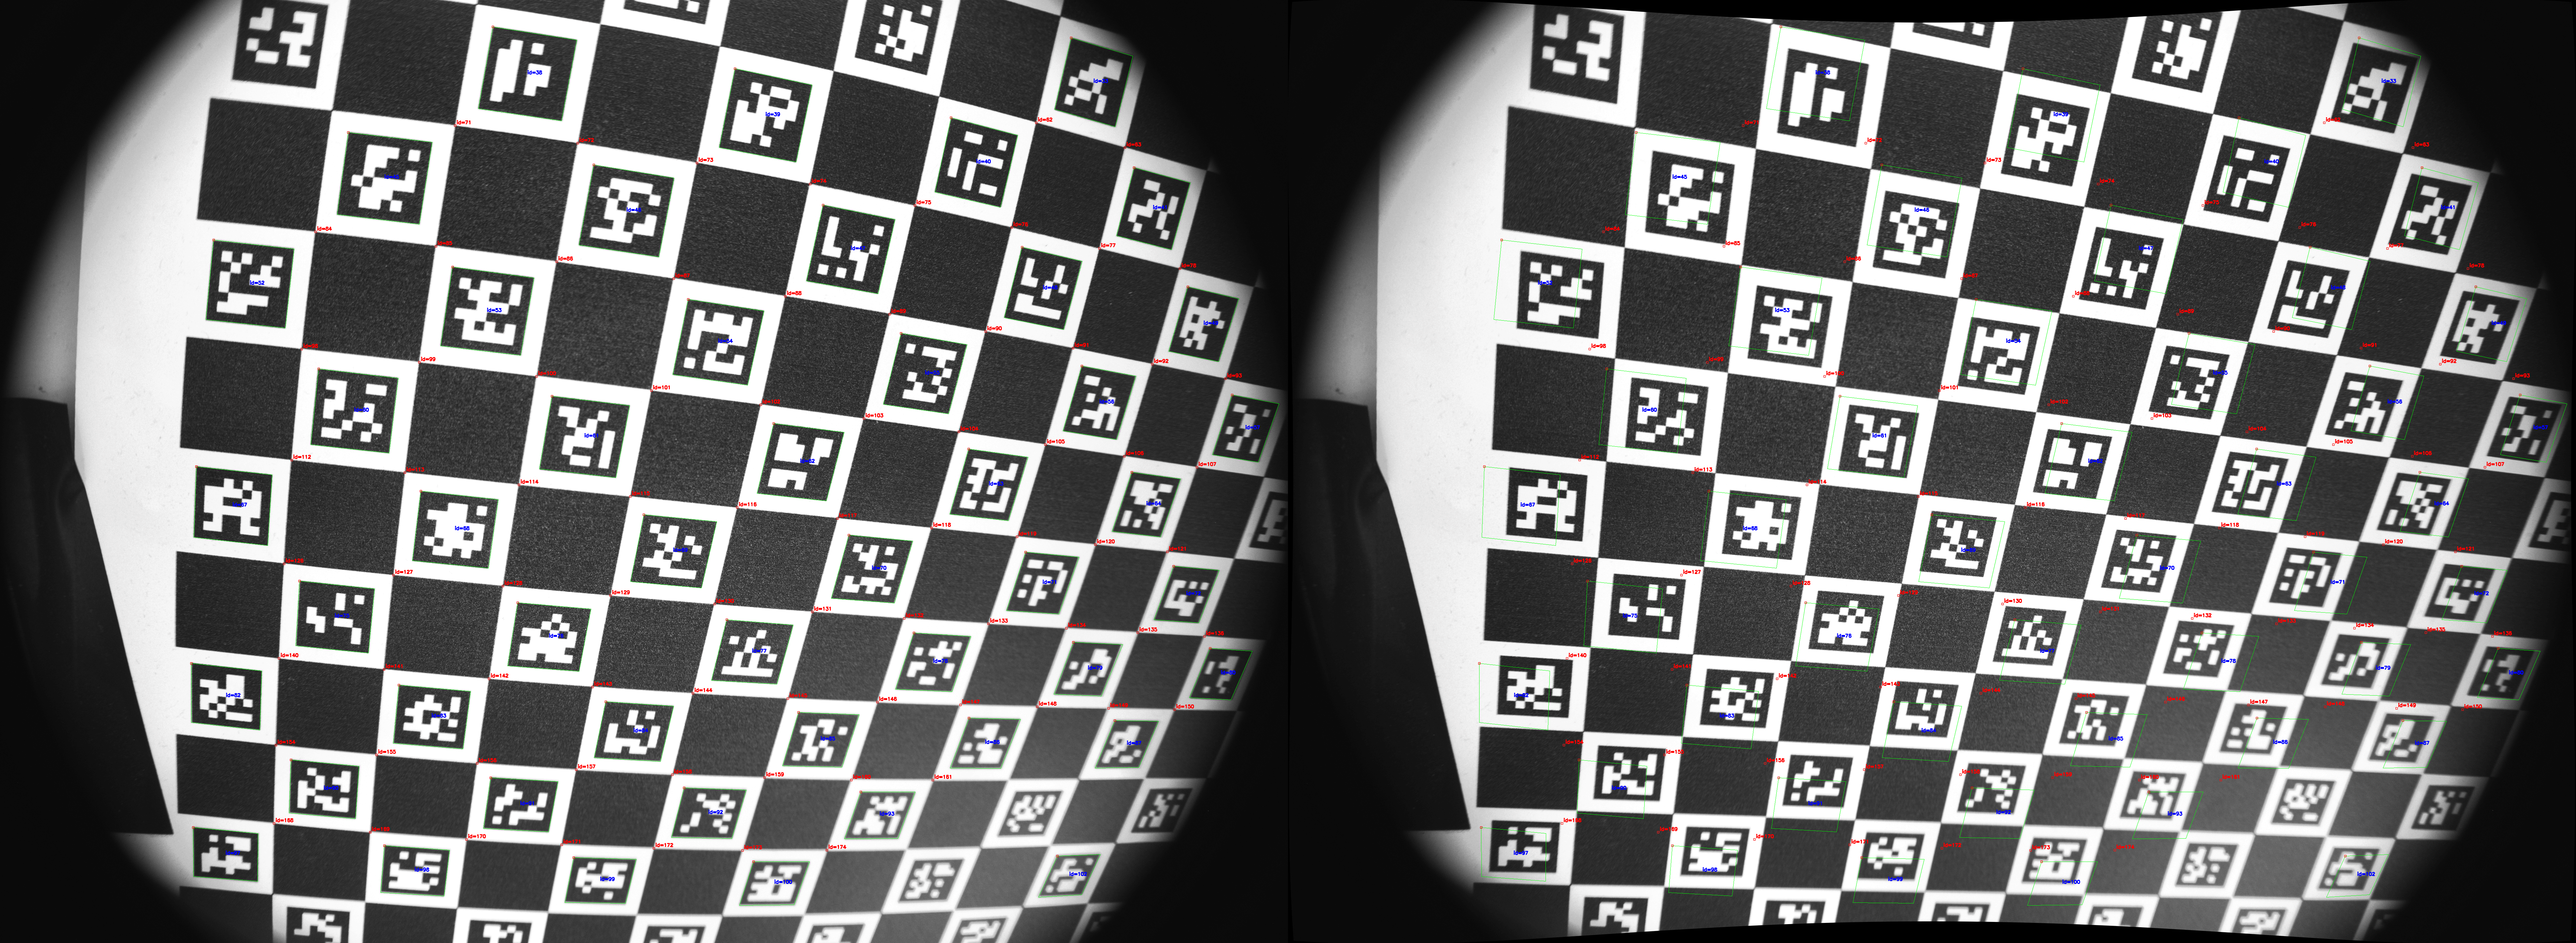
\includegraphics[width=0.75\linewidth]
	{images/chapter4Images/005_comparison_markers.png}
	\caption{Comparison between distorted and undistorted views of the ChArUco board after intrinsic calibration. The undistorted image shows corrected geometry and improved alignment of checkerboard corners and ArUco markers, validating the estimated intrinsic parameters.}
	\label{fig:charuco_undistortion}
\end{figure}


\begin{equation}
	\mathbf{K} =
	\begin{bmatrix}
		2448.06 & 0 & 655.98 \\
		0 & 2456.04 & 526.71 \\
		0 & 0 & 1
	\end{bmatrix}
\end{equation}

\begin{equation}
	\mathbf{d} =
	\begin{bmatrix}
		-0.4396 & 1.4435 & 9.06\times10^{-4} & 1.32\times10^{-3} & -6.0031
	\end{bmatrix}
\end{equation}


TODO add picture

% ��️ Two figures to add (both easy to generate from your own data)
% [IMG-12] — ChArUco detection image. Take any one of your calibration images and run it through OpenCV's cv::aruco::drawDetectedCornersCharuco() and cv::aruco::drawDetectedMarkers(). Save the result as a PNG and include it with:


%\begin{figure}[htbp]
%    \centering
%    \includegraphics[width=0.6\linewidth]{figures/charuco_detection.png}
%    \caption{Example of ChArUco corner detection on one calibration image.
%             Green dots mark the detected sub-pixel corners; coloured squares
%             show the detected ArUco markers with their IDs.}
%    \label{fig:charuco_detection}
%\end{figure}



TODO add figure
[IMG-13] — Intrinsic parameters table. Once you have your calibration results, fill in and add this table right before the last paragraph:
\begin{table}[htbp]
	\centering
	\caption{Intrinsic parameters of the Cognex CAM-CIC-12-9C-IP67 camera estimated via calibration.}
	\label{tab:intrinsics}
	\begin{tabular}{lll}
		\toprule
		\textbf{Parameter} & \textbf{Symbol} & \textbf{Value} \\
		\midrule
		Focal length (x) & $f_x$ & 2448.06 px \\
		Focal length (y) & $f_y$ & 2456.04 px \\
		Principal point x & $c_x$ & 655.98 px \\
		Principal point y & $c_y$ & 526.71 px \\
		\midrule
		Radial distortion & $k_1$ & -0.4396 \\
		Radial distortion & $k_2$ & 1.4435 \\
		Tangential distortion & $p_1$ & $9.06 \times 10^{-4}$ \\
		Tangential distortion & $p_2$ & $1.32 \times 10^{-3}$ \\
		Radial distortion & $k_3$ & -6.0031 \\
		\midrule
		\multicolumn{3}{l}{RMS reprojection error: \textbf{(add value here)} px} \\
		\bottomrule
	\end{tabular}
\end{table}

TODO
 Small optional upgrades (if you want later)

You can add:

1 image of Charuco detection (very good visually)

1 table with intrinsic parameters (fx, fy, cx, cy)



% ---------------------------------------------------------------
\section{Extrinsic Calibration}
\label{sec:extrinsic_calibration}
% ---------------------------------------------------------------

Extrinsic calibration estimates the rigid transformation $\mathbf{X} =
{}^E_C\mathbf{T} \in SE(3)$ between the robot end-effector frame $\{E\}$ and
the camera frame $\{C\}$. In the eye-in-hand configuration adopted in this
work (Section~\ref{subsec:eye_in_hand}), this transformation is fixed for
all robot configurations and constitutes the unknown quantity in the
hand-eye calibration equation~\eqref{eq:axxb}.

The extrinsic calibration pipeline combines:
\begin{enumerate}
    \item robot end-effector poses $\{{}^B_E\mathbf{T}^{(k)}\}$ from forward
    kinematics;
    \item camera-to-target poses $\{{}^C_T\mathbf{T}^{(k)}\}$ from
    PnP-based pose estimation;
    \item computation of relative motion pairs $(\mathbf{A}_{ij},
    \mathbf{B}_{ij})$;
    \item solution of $\mathbf{A}_{ij}\mathbf{X} = \mathbf{X}\mathbf{B}_{ij}$
    via \texttt{cv::calibrateHandEye()}.
\end{enumerate}

\noindent An overview of the pipeline is shown in
Figure~\ref{fig:extrinsic_pipeline}.

% ---------------------------------------------------------------
\subsection{Pose Estimation}
\label{subsec:extr_pose_est}
% ---------------------------------------------------------------

The camera-to-target transformation ${}^C_T\mathbf{T}^{(k)}$ at each robot
pose $k$ is estimated from the ChArUco corner correspondences using the
PnP formulation. The
intrinsic matrix $\mathbf{K}^*$ and distortion coefficients $\mathbf{d}^*$
obtained from the intrinsic calibration (Section~\ref{sec:intrinsic_calibration})
are passed as inputs to the PNP sover, which internally accounts for lens distortion.

The output of \texttt{cv::solvePnP()} at pose $k$ is a Rodrigues rotation
vector $\mathbf{r}^{(k)}$ and a translation vector ${}^C\mathbf{t}_T^{(k)}$,
which are assembled into the homogeneous transformation:

\begin{equation}
    {}^C_T\mathbf{T}^{(k)} =
    \begin{bmatrix}
        \mathbf{R}\!\left(\mathbf{r}^{(k)}\right) &
        {}^C\mathbf{t}_T^{(k)} \\
        \mathbf{0}^\top & 1
    \end{bmatrix} \in SE(3)
    \label{eq:CT_k}
\end{equation}

\noindent where $\mathbf{R}(\mathbf{r})$ is recovered via
Rodrigues' formula~\eqref{eq:rodrigues}. Each estimate
${}^C_T\mathbf{T}^{(k)}$ is validated against the reprojection error
threshold $\epsilon_{\max}$;
poses failing this criterion are excluded from the dataset.

% ---------------------------------------------------------------
\subsection{Construction of Motion Pairs}
\label{subsec:motion_pairs}
% ---------------------------------------------------------------

From the $n'$ validated observations, the relative motion pairs
$(\mathbf{A}_{ij}, \mathbf{B}_{ij})$ are computed for each pair of
distinct poses $(i, j)$ using equations~\eqref{eq:A_ij}--\eqref{eq:B_ij},
repeated here for clarity:

\begin{align}
    \mathbf{A}_{ij} &=
        \left({}^B_E\mathbf{T}^{(i)}\right)^{-1}
        {}^B_E\mathbf{T}^{(j)}
    \label{eq:A_ij_extr} \\[4pt]
    \mathbf{B}_{ij} &=
        {}^C_T\mathbf{T}^{(i)}
        \left({}^C_T\mathbf{T}^{(j)}\right)^{-1}
    \label{eq:B_ij_extr}
\end{align}

\noindent using the matrix inverse formula~\eqref{eq:T_inverse}.
$\mathbf{A}_{ij}$ encodes the relative motion of the end-effector in the
robot base frame; $\mathbf{B}_{ij}$ encodes the corresponding relative
motion of the camera as seen by the fixed target.

In preliminary experiments, using all possible motion-pair
combinations produced a large number of nearly redundant observations,
many of which corresponded to very small relative motions. Restricting
the dataset to consecutive observations reduced computational cost and
improved numerical conditioning while preserving sufficient motion
diversity for accurate calibration.

Each motion pair is further screened by computing the rotation angle of
$\mathbf{A}_{ij}$:

\begin{equation}
    \theta_{ij} = \arccos\!\left(
        \frac{\operatorname{tr}(\mathbf{R}_{A_{ij}}) - 1}{2}
    \right)
    \label{eq:rot_angle}
\end{equation}

\noindent Pairs with $\theta_{ij} < \theta_{\min}$ are discarded, as small
rotations do not constrain the rotational component
of~$\mathbf{X}$ \cite{strobl2006optimal}.

% ---------------------------------------------------------------

% ---------------------------------------------------------------
\subsection{Hand-Eye Calibration Methods}
\label{subsec:calib_methods}
% ---------------------------------------------------------------

The validated motion pairs
$\{(\mathbf{A}_{ij}, \mathbf{B}_{ij})\}$ are used to estimate the
fixed transformation between the robot end-effector frame and the
camera frame,

\begin{equation}
	\mathbf{X} = {}^E_C\mathbf{T},
\end{equation}

which satisfies the hand-eye calibration equation

\begin{equation}
	\mathbf{A}_{ij}\mathbf{X}
	=
	\mathbf{X}\mathbf{B}_{ij}.
\end{equation}

The calibration is performed using the OpenCV
\texttt{cv::calibrateHandEye()} implementation
\cite{bradski2008learning}, which provides several algorithms proposed
in the literature. The methods evaluated in this work are summarised in
Table~\ref{tab:hec_methods}.

\begin{table}[htbp]
	\centering
	\caption{Hand-eye calibration methods available in
		\texttt{cv::calibrateHandEye()} and evaluated in this work.}
	\label{tab:hec_methods}
	\begin{tabular}{llll}
		\toprule
		\textbf{Method} &
		\textbf{Reference} &
		\textbf{Formulation} &
		\textbf{Characteristics} \\
		\midrule
		Tsai--Lenz
		& \cite{tsai1989new}
		& Two-stage closed-form
		& Fast, robust, widely adopted \\
		Park--Martin
		& \cite{park1994robot}
		& Lie-group formulation
		& Numerically stable \\
		Horaud--Dornaika
		& \cite{horaud1995hand}
		& Simultaneous optimisation
		& Joint estimation of rotation and translation \\
		Andreff et al.
		& \cite{andreff1999online}
		& Linear matrix formulation
		& Suitable for online estimation \\
		Daniilidis
		& \cite{daniilidis1999hand}
		& Dual quaternion formulation
		& Simultaneous rigid-motion estimation \\
		\bottomrule
	\end{tabular}
\end{table}

Although all methods solve the same underlying
$\mathbf{A}\mathbf{X}=\mathbf{X}\mathbf{B}$ problem, they differ in how
rotation and translation are represented and estimated. Tsai--Lenz
computes rotation and translation separately, whereas Horaud--Dornaika
and Daniilidis estimate both simultaneously. Park--Martin formulates
the problem on the Lie group $SE(3)$ and is generally regarded as one
of the most numerically stable closed-form approaches.

In this work, all five algorithms are evaluated on the same dataset in
order to assess their robustness under realistic industrial operating
conditions. The comparison is performed using the validation metrics
introduced in before, and the quantitative
results are reported in Chapter~\ref{subsec:intrinsic_results}.

The OpenCV function call used throughout the experiments is shown below:

\begin{verbatim}
	cv::calibrateHandEye(
	R_gripper2base,
	t_gripper2base,
	R_target2cam,
	t_target2cam,
	R_cam2gripper,
	t_cam2gripper,
	method
	);
\end{verbatim}

where the inputs correspond to the robot poses
$\{{}^B_E\mathbf{T}^{(k)}\}$ and target poses
$\{{}^C_T\mathbf{T}^{(k)}\}$ obtained from the acquisition pipeline.
The selected method determines which calibration algorithm is used to
estimate the hand-eye transformation.

The resulting rotation matrix $\mathbf{R}_X$ and translation vector
$\mathbf{t}_X$ are assembled into the homogeneous transformation

\begin{equation}
	\hat{\mathbf{X}}
	=
	{}^E_C\hat{\mathbf{T}}
	=
	\begin{bmatrix}
		\mathbf{R}_X & \mathbf{t}_X \\
		\mathbf{0}^{\top} & 1
	\end{bmatrix}
	\in SE(3),
	\label{eq:X_estimated}
\end{equation}

which represents the estimated pose of the camera with respect to the
robot end-effector.

Preliminary experiments indicated that the Tsai--Lenz,
Park--Martin, and Horaud--Dornaika methods produced comparable
results, whereas the Andreff and Daniilidis formulations exhibited
greater sensitivity to noise in the estimated target poses. .



% ---------------------------------------------------------------
\subsection{Implementation Details}
\label{subsec:extr_implementation}
% ---------------------------------------------------------------

The extrinsic calibration pipeline was implemented in two stages.

\paragraph{Python prototype.}
The pipeline was first developed in Python using OpenCV
\cite{bradski2008learning}, enabling rapid evaluation of different pose
estimation strategies, calibration algorithms, and filtering thresholds.
The pseudocode in Algorithm~\ref{alg:extrinsic} summarises the complete
procedure.

\paragraph{C\# production implementation.}
Once validated, the pipeline was ported to C\# for integration within the
\textit{Cognex Designer} industrial vision environment. This step embeds
the calibration directly into the production vision workflow, enabling
evaluation under realistic industrial operating conditions. Particular
attention was given to maintaining consistent coordinate frame conventions
between the Python prototype and the C\# implementation, as sign errors in
frame conventions are a common source of systematic calibration error.

\paragraph{Calibration validation interface.}
To verify the estimated transformation $\hat{\mathbf{X}} = {}^E_C\hat{\mathbf{T}}$
under realistic acquisition conditions, a point transformation demonstrator
was developed within the same \textit{Cognex Designer} environment. The tool
accepts live images directly from the Cognex CAM-CIC-12-9C-IP67 camera and
robot pose data in XYZWPR format from a user-supplied CSV file, and allows
the operator to select an arbitrary image point $(u, v)$ and receive its
corresponding coordinates in the robot base frame $\{B\}$.

The transformation chain applied is:

\begin{equation}
	{}^B\mathbf{P} =
	{}^B_E\mathbf{T} \cdot {}^E_C\hat{\mathbf{T}} \cdot
	\pi^{-1}\!\left(\mathbf{K}^*,\, \mathbf{d}^*,\, u,\, v,\, Z\right)
	\label{eq:pixel_to_base}
\end{equation}

\noindent where $\pi^{-1}(\cdot)$ denotes the back-projection of the image
point $(u,v)$ into a 3D ray in the camera frame, evaluated at a working
distance $Z$ measured along the optical axis. Since a single image point
defines a ray rather than a unique 3D point, $Z$ is treated as a known
constant corresponding to the nominal distance between the camera and the
calibration plane. The robot pose ${}^B_E\mathbf{T}$ is constructed from
the XYZWPR values provided by the user, following the FANUC convention for
end-effector pose representation.

This interface serves as a qualitative end-to-end validation of the full
calibration pipeline: geometric consistency between the predicted base-frame
coordinates and the known physical layout of the scene confirms that the
estimated $\hat{\mathbf{X}}$ is correct in both rotation and translation.

\begin{algorithm}
	\caption{Extrinsic hand-eye calibration pipeline}
	\label{alg:extrinsic}
	\begin{algorithmic}[1]
		\Require Robot poses $\{{}^B_E\mathbf{T}^{(k)}\}_{k=1}^{n}$,
		calibration images $\{\mathcal{I}^{(k)}\}_{k=1}^{n}$,
		intrinsics $(\mathbf{K}^*, \mathbf{d}^*)$,
		thresholds $m_{\min}$, $\epsilon_{\max}$, $\theta_{\min}$
		\Ensure  Estimated transformation $\hat{\mathbf{X}} = {}^E_C\hat{\mathbf{T}}$
		
		\State $\mathcal{D} \leftarrow \emptyset$
		\Comment{Initialise validated observation dataset}
		\For{$k = 1$ \textbf{to} $n$}
		\State Detect ChArUco corners in $\mathcal{I}^{(k)}$; obtain $m_k$ corners
		\If{$m_k < m_{\min}$} \textbf{continue} \EndIf
		\State Estimate ${}^C_T\mathbf{T}^{(k)}$ via \texttt{solvePnP()}
		\If{$\bar{\epsilon}^{(k)} > \epsilon_{\max}$} \textbf{continue} \EndIf
		\State $\mathcal{D} \leftarrow \mathcal{D} \cup
		\bigl\{\bigl({}^B_E\mathbf{T}^{(k)},\;
		{}^C_T\mathbf{T}^{(k)}\bigr)\bigr\}$
		\EndFor
		
		\State $\mathcal{P} \leftarrow \emptyset$
		\Comment{Initialise validated motion pair set}
		\For{each consecutive pair $(i,\, i{+}1)$ in $\mathcal{D}$}
		\State Compute $\mathbf{A}_{i,i+1}$ via~\eqref{eq:A_ij_extr}
		\State Compute $\theta_{i,i+1}$ via~\eqref{eq:rot_angle}
		\If{$\theta_{i,i+1} < \theta_{\min}$} \textbf{continue} \EndIf
		\State Compute $\mathbf{B}_{i,i+1}$ via~\eqref{eq:B_ij_extr}
		\State $\mathcal{P} \leftarrow \mathcal{P} \cup
		\{(\mathbf{A}_{i,i+1},\, \mathbf{B}_{i,i+1})\}$
		\EndFor
		
		\For{\textbf{each} method $\in$
			\{\textsc{Tsai}, \textsc{Park}, \textsc{Horaud},
			\textsc{Andreff}, \textsc{Daniilidis}\}}
		\State $\hat{\mathbf{X}}_{\text{method}} \leftarrow$
		\texttt{calibrateHandEye}$(\mathcal{P},\; \text{method})$
		\State Verify translation component via
		Kabsch--Umeyama alignment~\eqref{eq:kabsch_obj}
		\State Evaluate $\hat{\mathbf{X}}^*_{\text{method}}$ using
		validation metrics
		\EndFor
		
		\State \Return $\hat{\mathbf{X}}^*$ with lowest validation error
		
	\end{algorithmic}
\end{algorithm}

\begin{figure}[htbp]
    \centering
    \begin{tikzpicture}[
        node distance  = 0.5cm and 1.5cm,
        box/.style     = {draw, rounded corners=5pt, minimum width=3.6cm,
                          minimum height=0.85cm, align=center, font=\small},
        source/.style  = {box, fill=blue!8},
        process/.style = {box, fill=orange!10},
        output/.style  = {box, fill=green!10, font=\small\bfseries},
        arr/.style     = {-Stealth, thick},
        lbl/.style     = {font=\footnotesize, fill=white, inner sep=1pt},
    ]

    % --- Left branch: robot ---
    \node[source]  (robot) {Robot controller\\
                            \footnotesize joint readings $\mathbf{q}^{(k)}$};
    \node[process, below=of robot] (fk) {Forward kinematics\\
                            \footnotesize ${}^B_E\mathbf{T}^{(k)}$};

    % --- Right branch: vision ---
    \node[source,  right=2.8cm of robot] (cam) {Camera image\\
                            \footnotesize $\mathcal{I}^{(k)}$};
    \node[process, below=of cam]  (det) {ChArUco detection\\
                            \footnotesize \texttt{detectBoard()}};
    \node[process, below=of det]  (pnp) {Pose estimation (PnP)\\
                            \footnotesize ${}^C_T\mathbf{T}^{(k)}$};

    % --- Centre merge: motion pairs ---
    \node[process, below=2.1cm of fk,
          xshift=2.3cm]           (pair){Motion pair computation\\
                            \footnotesize
                            $\mathbf{A}_{ij}$,\; $\mathbf{B}_{ij}$};

    % --- Output: calibrateHandEye ---
    \node[output,  below=0.7cm of pair] (hec) {\texttt{calibrateHandEye()}\\
                            \footnotesize Tsai, Park, Horaud,
                            Andreff, Dtaniilidis};
    \node[output,  below=0.6cm of hec]  (X)   {$\hat{\mathbf{X}} =
                            {}^E_C\hat{\mathbf{T}}$};

    % --- Arrows ---
    \draw[arr] (robot) -- (fk);
    \draw[arr] (cam)   -- (det);
    \draw[arr] (det)   -- (pnp);
    \draw[arr] (fk.south)  |- (pair.west);
    \draw[arr] (pnp.south) |- (pair.east);
    \draw[arr] (pair)  -- (hec);
    \draw[arr] (hec)   -- (X);

    % --- Repeat loop label ---
    \draw[arr, dashed, gray]
        (X.east) -- ++(0.8,0) |- node[lbl, right]{repeat for each $k$}
        (robot.east);
    \end{tikzpicture}
    \caption{Extrinsic calibration pipeline. Robot kinematics and
             vision-based pose estimation provide the motion pairs
             $(\mathbf{A}_{ij}, \mathbf{B}_{ij})$, which are passed to
             \texttt{cv::calibrateHandEye()} to estimate the unknown
             transformation $\hat{\mathbf{X}} = {}^E_C\hat{\mathbf{T}}$.}
    \label{fig:extrinsic_pipeline}
\end{figure}



TODO
1. Add a small diagram

Flow:

Robot Pose → A  
Images → solvePnP → B  
A, B → calibrateHandEye → X


2. Add one code snippet (optional)

Even pseudo-code:

for each image:
    detect corners
    estimate pose
compute A, B
run calibrateHandEye





% ---------------------------------------------------------------
\section{Improvements and Refinements}
\label{sec:improvements}
% ---------------------------------------------------------------

While the baseline calibration pipeline described in
Section~\ref{sec:extrinsic_calibration} provides a complete solution to the
hand-eye calibration problem, its performance in real-world industrial
environments is strongly influenced by measurement noise, detection errors, and
the quality of the acquired data. For this reason, several refinement strategies
have been introduced in order to improve the robustness, accuracy, and
repeatability of the estimated transformation $\hat{\mathbf{X}}$.

These enhancements target three aspects of the pipeline: rigid transformation
refinement via the Kabsch--Umeyama algorithm, systematic pose diversity during acquisition, and
reprojection-error-based data filtering.

A key finding of this work is that \textit{the quality of the calibration
depends more strongly on the quality and diversity of the input data than on
the choice of the hand-eye algorithm itself}. This motivates the emphasis
placed on data selection and refinement throughout this chapter.

% ---------------------------------------------------------------
\subsection{Rigid Transformation Refinement: Kabsch--Umeyama Method}
\label{subsec:kabsch}
% ---------------------------------------------------------------

A primary source of error in the calibration pipeline is noise in the
translation component of the PnP pose estimates ${}^C_T\mathbf{T}^{(k)}$.
While outlier filtering removes
grossly incorrect estimates, residual noise in accepted poses still degrades
the calibration. To mitigate this, a refinement step based on the
\textit{Kabsch--Umeyama algorithm} \cite{umeyama1991least} is applied.

Given two sets of $n$ corresponding 3D points $\{\mathbf{x}_i\} \subset
\mathbb{R}^3$ and $\{\mathbf{y}_i\} \subset \mathbb{R}^3$, the
Kabsch--Umeyama algorithm finds the rigid transformation
$(\mathbf{R}^*, \mathbf{t}^*) \in SE(3)$ minimising the mean squared
alignment error:


TODO check argmin
\begin{equation}
    (\mathbf{R}^*, \mathbf{t}^*) =
    \operatorname*{arg\,min}_{\mathbf{R} \in SO(3),\, \mathbf{t} \in \mathbb{R}^3}
    \frac{1}{n} \sum_{i=1}^{n}
    \left\lVert \mathbf{y}_i -
    \left(\mathbf{R}\mathbf{x}_i + \mathbf{t}\right) \right\rVert^2
    \label{eq:kabsch_obj}
\end{equation}

\noindent The closed-form solution is obtained via singular value decomposition
(SVD) of the cross-covariance matrix \cite{umeyama1991least}:

\begin{equation}
    \boldsymbol{\Sigma}_{xy} =
    \frac{1}{n} \sum_{i=1}^{n}
    (\mathbf{y}_i - \boldsymbol{\mu}_y)
    (\mathbf{x}_i - \boldsymbol{\mu}_x)^{\top}
    = \mathbf{U} \mathbf{\Lambda} \mathbf{V}^{\top}
    \label{eq:kabsch_svd}
\end{equation}

\noindent where $\boldsymbol{\mu}_x = \frac{1}{n}\sum_i \mathbf{x}_i$ and
$\boldsymbol{\mu}_y = \frac{1}{n}\sum_i \mathbf{y}_i$ are the centroids.
The optimal rotation and translation are then:

\begin{align}
    \mathbf{R}^* &= \mathbf{U}\,
        \operatorname{diag}(1, 1, \det(\mathbf{U}\mathbf{V}^{\top}))\,
        \mathbf{V}^{\top}
    \label{eq:kabsch_R} \\
    \mathbf{t}^* &= \boldsymbol{\mu}_y - \mathbf{R}^* \boldsymbol{\mu}_x
    \label{eq:kabsch_t}
\end{align}

\noindent The sign correction $\det(\mathbf{U}\mathbf{V}^{\top})$ in
equation~\eqref{eq:kabsch_R} ensures that $\mathbf{R}^* \in SO(3)$ (i.e.\
$\det(\mathbf{R}^*) = +1$) even when the data is severely corrupted, which
is the key improvement of Umeyama's formulation over earlier SVD-based methods
\cite{umeyama1991least}.

In the context of this work, the Kabsch--Umeyama method is applied as a
post-processing step. The translation vectors
$\{{}^C\mathbf{t}_T^{(k)}\}$ extracted from the validated pose estimates
${}^C_T\mathbf{T}^{(k)}$ are treated as one point set, and the corresponding
end-effector positions $\{{}^B\mathbf{t}_E^{(k)}\}$ as the other. Aligning
these two point clouds in a least-squares sense provides a geometrically
consistent estimate of the translational component of of the estimated transformation, which
is used to initialise or verify the output of \texttt{calibrateHandEye()}.
This is particularly effective at reducing the effect of outliers that survive
the reprojection error threshold but still introduce bias in the translation
estimate.


During the experimental evaluation, this refinement and consistency analysis
also proved useful for identifying small systematic geometric errors in the
physical setup. In particular, the ChArUco board — intended to be horizontally
aligned with the robot workspace — was found to exhibit a slight inclination
of approximately $0.5^\circ$--$1^\circ$. Although such a tilt does not prevent
corner detection or P$n$P pose estimation, it introduces a consistent geometric
bias across observations, which propagates into the estimated camera-to-target
transformations and consequently affects the hand-eye calibration result.

The alignment residuals obtained after the Kabsch--Umeyama refinement made
this systematic deviation observable, allowing the physical setup to be
corrected and improving the stability of the estimated transformation
$\mathbf{X} = {}^E_C\mathbf{T}$.

% ---------------------------------------------------------------
 ---------------------------------------------------------------
\subsection{Pose Selection and Motion Diversity}
\label{subsec:pose_selection}
% ---------------------------------------------------------------

The conditioning of the hand-eye calibration problem depends directly on the
geometric diversity of the collected motion pairs
\cite{strobl2006optimal, park1994robot}. Formally, the calibration equation
system~\eqref{eq:axxb} is well-conditioned if and only if the rotation axes of
the collected $\mathbf{A}_{ij}$ are not all parallel
(Section~\ref{subsec:observability}).

In this work, pose selection is performed manually during data acquisition
following a structured protocol:

\begin{itemize}
    \item \textbf{Axis diversity:} the end-effector is reoriented around
    at least three non-parallel axes, ensuring that the rotation axes of
    consecutive motion pairs $\mathbf{A}_{i,i+1}$ span $\mathbb{R}^3$.

    \item \textbf{Rotation magnitude:} each motion involves a rotation of at
    least $\theta_{\min} = 15^{\circ}$, checked via
    equation~\eqref{eq:rot_angle}, to avoid near-identity matrices
    $\mathbf{A}_{ij} \approx \mathbf{I}$.

    \item \textbf{Spatial distribution:} the end-effector is moved to
    positions distributed across the reachable workspace, providing a wide
    range of viewpoints on the calibration target.

    \item \textbf{Degenerate motions excluded:} pure translations
    ($\mathbf{R}_{A_{ij}} = \mathbf{I}$) and rotations around a single
    repeated axis are explicitly avoided.
\end{itemize}









% TODO

%  Optional upgrades (if you want to go one level higher)

% If you want to impress your professor, we can add:

% 1. One figure

% Before/after filtering (reprojection error plot)

% 2. One small table

% Dataset before filtering vs after filtering

% 3. One strong sentence (very thesis-like)

% Something like:

% “Experimental results demonstrate that data filtering and pose diversity have a greater impact on calibration accuracy than the choice of the hand-eye algorithm itself.”

% ��️ Two figures to generate from your own data
% [IMG-14] — Reprojection error before/after filtering (fig:reproj_before_after). Plot the per-image ϵˉ(i)\bar{\epsilon}^{(i)}
% ϵˉ(i) as a bar chart, with accepted images in blue and rejected ones in red, before and after applying the threshold. You can generate this in Python with
% matplotlib directly from your calibration output. This is the single most impactful figure you can add to this section.
% [IMG-15] — Multi-stage filtering pipeline (fig:filtering_pipeline). A simple three-box vertical flowchart (Intrinsic filtering → PnP filtering → Rotation angle screening) showing at each stage how many images/pairs enter and how many survive. Numbers from your actual dataset will make this very concrete for the examiner.